\documentclass[11pt]{book}
\usepackage{geometry}        
\geometry{letterpaper}    
\usepackage[parfill]{parskip}  
\usepackage{graphicx}
\usepackage{amssymb}
\usepackage{epstopdf}

\DeclareGraphicsRule{.tif}{png}{.png}{`convert #1 `dirname #1`/`basename #1 .tif`.png}

\usepackage[colorlinks=true, pdfstartview=FitV, linkcolor=blue, 
            citecolor=blue, urlcolor=blue]{hyperref}

%\includeonly{Chapter1}
\usepackage{geometry}                		% See geometry.pdf to learn the layout options. There are lots.
\geometry{letterpaper}    
\usepackage{graphicx}
  \usepackage{ams math}
  \usepackage{tikz}
 \usepackage{tcolorbox}
 \tcbuselibrary{skins}
 \tcbuselibrary{theorems}
\usepackage{hyperref}   
\usepackage{color}
\newcommand{\VAR}{CTRL-r }
%\usepackage[dvipsnames]{xcolor}
         		% ... or a4paper or a5paper or ... 
%\geometry{landscape}                		% Activate for for rotated page geometry
%\usepackage[parfill]{parskip}    		% Activate to begin paragraphs with an empty line rather than an indent
\usepackage{graphicx}				% Use pdf, png, jpg, or eps§ with pdflatex; use eps in DVI mode
								% TeX will automatically convert eps --> pdf in pdflatex		
\usepackage{amssymb}


%\author{The Author}
%\date{}							% Activate to display a given date or no date
%\newcommand{\inp}[1]{\texttt{\colorbox{yellow!25}{#1}}}
\newcommand{\inp}[1]{\begin{tcolorbox}[colback=yellow!25!,colframe=black]\texttt{#1} \end{tcolorbox}}

%\newcommand{\proc}[1]{\texttt{\colorbox{green!25}{#1}}}
\newcommand{\proc}[1]{\begin{tcolorbox}[colback=green!35!white,colframe=black]#1 \end{tcolorbox}}
 
 \newcommand{\coqtwo}[2]{
 \begin{tcolorbox}[bicolor,righthand width=\linewidth/4,sidebyside,colback=green!35!white,colbacklower=gray!10!white] {\small \texttt{#1}}\tcblower
$#2$ \end{tcolorbox}}
 
\newcommand{\coq}[1]{\begin{tcolorbox}[colback=gray!10!white,colframe=black]$#1$ \end{tcolorbox}}
\newcommand{\mess}[1]{\begin{tcolorbox}[colback=white,colframe=black] #1 \end{tcolorbox}}
\newtheorem{Theorem}{Theorem}
\newtheorem{Lemma}{Lemma}
\newtheorem{Proposition}{Proposition}
\newtheorem{Definition}{Definition}
\newtheorem{Axiom}{Axiom}
\tcbuselibrary{breakable}


\newtheorem{theorem}{Theorem}
\newtheorem{corollary}[theorem]{Corollary}
\newtheorem{definition}{Definition}
\newtheorem{lemma}{Lemma}
\newtheorem{exercise}{Exercise}
\newtheorem{remark}{Remark}
\newtheorem{example}{Example}
\newtheorem{warning}{Warning}
\usepackage{subfiles}
\def\grad{ \mbox{grad}}
\def\curl{ \mbox{curl}}
\def\div{ \mbox{div}}
\def\U{\ensuremath {\cal U}}
\def\S{\ensuremath {\cal S}}
\def\V{\ensuremath {\cal V}}
\def\R{\ensuremath {\cal R}}
\def\tr{\ensuremath {\mbox{tr}}}




% ------------------- Title and Author -----------------------------
\title{Sample Book}
\author{Author}
\begin{document}


\frontmatter
\maketitle

\tableofcontents


\section{ Installation}

\subsection{Mac OSX}
\begin{enumerate}
\item Download and install  the latest version of Coq (it needs to be at least 8.6) from :

\href{https://coq.inria.fr/download}{https://coq.inria.fr/download}

Move it to your apps folder.


\item  Download and unpack spatchocq.app from canvas
move the spatchcoq.app to Applications and start it. 

\item when prompted find the Coq installation you have just move above. Navigate to 
\begin{verbatim}
/Applications/CoqIDE_8.6.app/Contents/Resources/bin/
\end{verbatim}
and choose coqtop. See Figure~\ref{fig:macos}

You only do this once.
\item  You only have to do this once. You might also need to install gtk, the simplest way to do this is  via homebrew
{\center brew install gtk+}
\begin{figure}\label{fig:macos}
\center
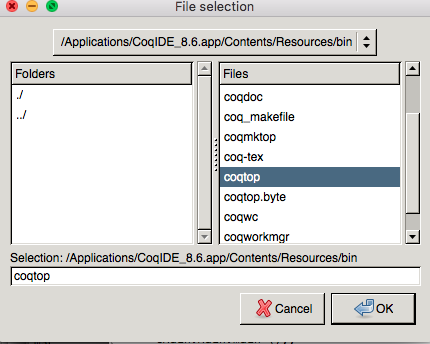
\includegraphics[scale=0.5]{Installation/macos.png}
\caption{Choose the Coq app in a Mac env}\label{fig:macos}
\end{figure}
\item enjoy

\end{enumerate}

\subsection{Windows}
\begin{enumerate}

\item get the zipfile spatchcoq.zip,  unzip it in a folder on a usb stick and doubleclick the application file spatchcoq. 
Note this version includes an instalation of Coq (not very extensively tested yet)

\item enjoy
\end{enumerate}


\subsection{Linux}
\begin{enumerate}
\item Download and install  the latest version of Coq it needs to be at least 8.6 so do not use 
apt-get install coq
\item  go to https://github.com/corneliuhoffman/spatchcoqocaml/tree/master
to build from scratch.
\item when prompted go to the Coq folder you just installed with opam and find  the application called {\bf coqtop}

\item enjoy
\end{enumerate}











\subfile{Tactics/tactics}


\bibliographystyle{plain-annote}
\bibliography{mybibliography}



\end{document}
\end

